
% # COPYRIGHT:
%
%   Copyright (C)  2011 Jeremiah Mahler <jmmahler@gmail.com>.
%   Permission is granted to copy, distribute and/or modify this document
%   under the terms of the GNU Free Documentation License, Version 1.3
%   or any later version published by the Free Software Foundation;
%   with no Invariant Sections, no Front-Cover Texts, and no Back-Cover Texts.
%   A copy of the license is included in the file "fdl-1.3.txt".
%

\documentclass[12pt]{article}
%\documentclass[10pt]{article}

%\usepackage{mslapa}
\usepackage{hyperref}
\usepackage{amsmath}
\usepackage{graphicx}
\usepackage{ulem}
\usepackage{vmargin}
\usepackage{tabularx}
\usepackage{sectsty}
\usepackage{pbox}
\usepackage{bigstrut}
\usepackage{enumerate}
\usepackage{parskip}  % add spaces between paragraphs
\input kvmacros  % Karnaugh Maps and Veitch charts

%\usepackage{cleveref}

%\setpapersize{USletter}
\sectionfont{\normalsize}
\subsectionfont{\normalsize}

% configure \bigstrut size
% This configures spacing above and below rows in a tabularx.
%\renewcommand{\bigstrutjot}{6pt}
\renewcommand{\bigstrutjot}{2.0\jot}

\setlength{\parindent}{0in}

\raggedright

\begin{document}

% {{{ Cover Page

\centerline{\bf EECE 144}
\centerline{\bf Fall 2011}
\centerline{\bf}
\centerline{\bf Lab Report \#7}
\centerline{\bf Section 4}
\centerline{\bf 10/19/2011}

% signature area
\begin{center}
\begin{tabularx}{\textwidth}[b]{X l l}
Submitted by: Jeremiah Mahler & & \\
Signature & Printed Name & Date \\
\hline
\multicolumn{1}{|X|}{} & \multicolumn{1}{|l|}{\bigstrut \bf Jeremiah Mahler} & \multicolumn{1}{|l|}{\bf Oct 19, 2011} \\
\hline
\multicolumn{1}{|X|}{} & \multicolumn{1}{|l|}{\bigstrut \bf Marvanee Johnson} & \multicolumn{1}{|l|}{\bf Oct 19, 2011} \\
\hline
\end{tabularx}
\end{center}
% }}}

\section{Description/Objectives}

% description
The objective of this lab is to develop an optimized hardware
implementation of two distinct logic functions
(Equation \ref{eq:Jcsop} and \ref{eq:Kcsop}).
First the logic functions will be analyzed/optimized individually.
Then they will be combined in to a jointly optimized solution.
The jointly optimized solution will then be implemented in hardware
using 74HC04(NOT), 74HC08(AND), and 74HC32(OR) gates.

% (objective)
Once completed it should be possible to confirm that the jointly
optimized solution behaves identically to the singly optimized solution.

\begin{align}
J(w, x, y, z) &= \sum m(1,3,9,11,12,13,14,15) \label{eq:Jcsop} \\
K(w, x, y, z) &= \sum m(0,1,3,12,14) \label{eq:Kcsop}
\end{align}

\section{Procedure}
\label{sec:procedure}

\begin{samepage}
The procedure consists of several steps:
\begin{enumerate}
	\item Find the minimal SOP expression of $J$ and $K$ separately
	using Karnaugh maps.
	\item Calculate the number of gates and number of gate inputs required
	to implement these functions using gates with any number of inputs.
	\item Calculate the number of gates and number of gate inputs required
	to implement these functions using only two input gates.
	\item Find a jointly optimized solution of $J$ and $K$ which minimizes
	the number of gates using Karnaugh maps.
	\item Calculate the number of gates and number of gate inputs required
	to implement this function using only two input gates.
	\item Implement the jointly optimized function in hardware and verify
	it against a truth table of the original functions (Table \ref{tbl:tt}).
\end{enumerate}
\end{samepage}

\begin{table}[htb]
\begin{center}
\begin{tabular}{lr}
  \begin{tabular}[t]{r|cccc|c|c}
  Index&$w$&$x$&$y$&$z$&$J$&$K$\\
  \hline
  0  &0&0&0&0 &0 &1\\
  1  &0&0&0&1 &1 &1\\
  2  &0&0&1&0 &0 &0\\
  3  &0&0&1&1 &1 &1\\
  4  &0&1&0&0 &0 &0\\
  5  &0&1&0&1 &0 &0\\
  6  &0&1&1&0 &0 &0\\
  7  &0&1&1&1 &0 &0\\
  8  &1&0&0&0 &0 &0\\
  9  &1&0&0&1 &1 &0\\
  10 &1&0&1&0 &0 &0\\
  11 &1&0&1&1 &1 &0\\
  12 &1&1&0&0 &1 &1\\
  13 &1&1&0&1 &1 &0\\
  14 &1&1&1&0 &1 &1\\
  15 &1&1&1&1 &1 &0\\
  \end{tabular}
\end{tabular}
\end{center}
\caption{Truth table of functions $J$ and $K$.}
\label{tbl:tt}
\end{table}

\begin{samepage}
The first step is to find a minimal SOP expression for $J$.
Using the Karnaugh map for $J$ (Figure \ref{fig:Jmap})
results in two prime implicants as shown in Equation \ref{eq:Jsop}.

\begin{equation}
	J = w x + x' z  \label{eq:Jsop}
\end{equation}
\end{samepage}

\begin{figure}[!hbt]
\begin{center}
\karnaughmap{4}{$J(w,x,y,z)$:}{wxyz}{0101000001011111}{}
\end{center}
\caption{Karnaugh map of function $J$ (Equation \ref{eq:Jcsop}).}
\label{fig:Jmap}
\end{figure}

Similarly, finding a minimal SOP expression for $K$ using its
Karnaugh map (Figure \ref{fig:Kmap}) results in three prime implicants
as shown in Equation \ref{eq:Ksop}.

\begin{figure}[!hbt]
\begin{center}
\karnaughmap{4}{$K(w,x,y,z)$:}{wxyz}{1101000000001010}{}
\end{center}
\caption{Karnaugh map of function $K$ (Equation \ref{eq:Kcsop}).}
\label{fig:Kmap}
\end{figure}

\begin{equation}
	K = w'x'y' + w'x'z + wxz'  \label{eq:Ksop}
\end{equation}

A gifted mind of electronics can probably deduce the number of
gates and gate inputs from the expressions alone.
But here we appeal to the not so brilliant of us by using
circuit diagrams to clearly elucidate the metrics we
are seeking.

Referring to the circuit for $J$ in Figure \ref{fig:Jminsop-01} we
can see that there are 2 AND gates, 1 OR gate, and 1 NOT gate.
And there are 4 inputs to the AND gates, 2 inputs to the OR gate,
and 1 input to the NOT gate.

\begin{figure}[htb]
\center
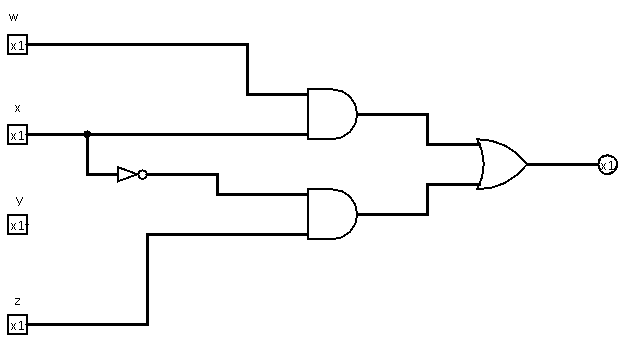
\includegraphics[scale=0.5]{Jminsop-01}
\caption{Circuit diagram of the minimal SOP solution of $J$.}
\label{fig:Jminsop-01}
\end{figure}

Referring to the circuit for $K$ in Figure \ref{fig:Kminsop-01} we
can see that there are 3 AND gates, 1 OR gate and 4 NOT gates.
And there are 9 inputs to the AND gates, 3 inputs to the OR gate,
and 4 inputs to the NOT gates.

\begin{figure}[!htb]
\center
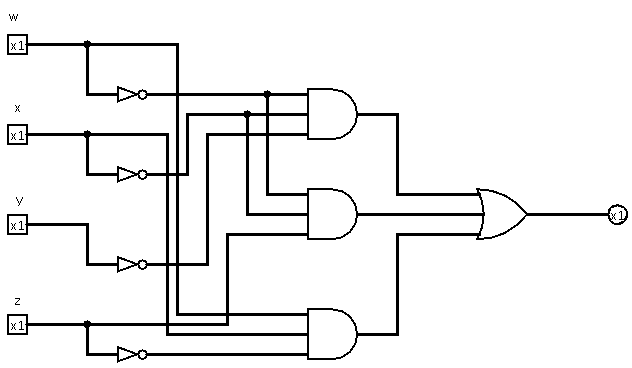
\includegraphics[scale=0.5]{Kminsop-01}
\caption{Circuit diagram of the minimal SOP solution of $K$.}
\label{fig:Kminsop-01}
\end{figure}

When limited to two gates the previous solution for $J$ is the
same.
For $K$ the circuit must be modified as shown in Figure \ref{fig:Kminsop-02}.
There are 4 NOT gates, 6 AND gates and 2 OR gates.
And there are 4 inputs to the NOT gates, 12 inputs to the AND gates,
and 4 inputs to the OR gates.

\begin{figure}[!htb]
\center
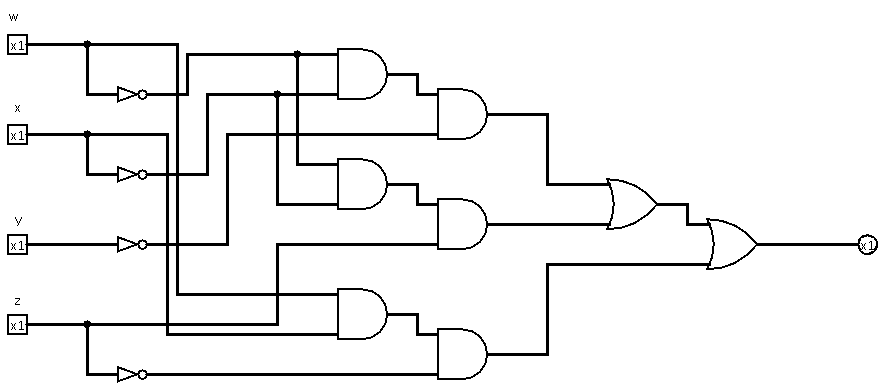
\includegraphics[scale=0.5]{Kminsop-02}
\caption{Circuit diagram of the minimal SOP solution of $K$ when limited to two input gates.}
\label{fig:Kminsop-02}
\end{figure}

\clearpage

Jointly optimizing both $J$ and $K$ together is somewhat more complex than
either individually.
The general strategy is to find essential prime implicants and then to find
implicants which are common to both functions.

Figure \ref{fig:JKjointkmap} shows the implicants in a Karnaugh map
of a jointly optimized solution.
And Equation \ref{eq:JKjoint} is the resulting expressions.

\begin{align}
	J &= w'x'z + wxz' + wz  \notag \\
	K &= w'x'z + wxz' + w'x'y'  \label{eq:JKjoint}
\end{align}

\begin{figure}[!htb]
\center
%\karnaughmap{4}{$J(w,x,y,z)$:}{wxyz}{0101000001011111}{}
%\karnaughmap{4}{$K(w,x,y,z)$:}{wxyz}{1101000000001010}{}
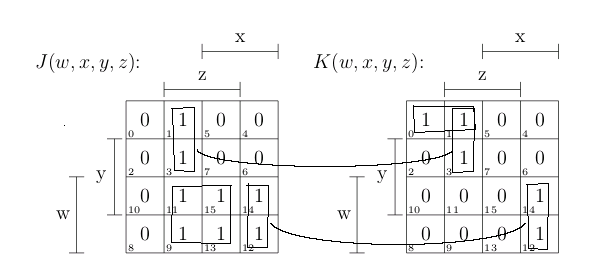
\includegraphics[scale=0.60]{JKkmap-01}
\caption{Jointly optimized Karnaugh maps for $J$ and $K$.}
\label{fig:JKjointkmap}
\end{figure}

And the circuit diagram of the jointly optimized solution is given
in Figure \ref{fig:JKjointcircuit}.
It can be seen that there are 4 NOT gates, 7 AND gates and 4 OR gates.
There are 4 NOT gate inputs, 14 AND gate inputs, and 8 OR gate inputs.

\begin{figure}[!htb]
\center
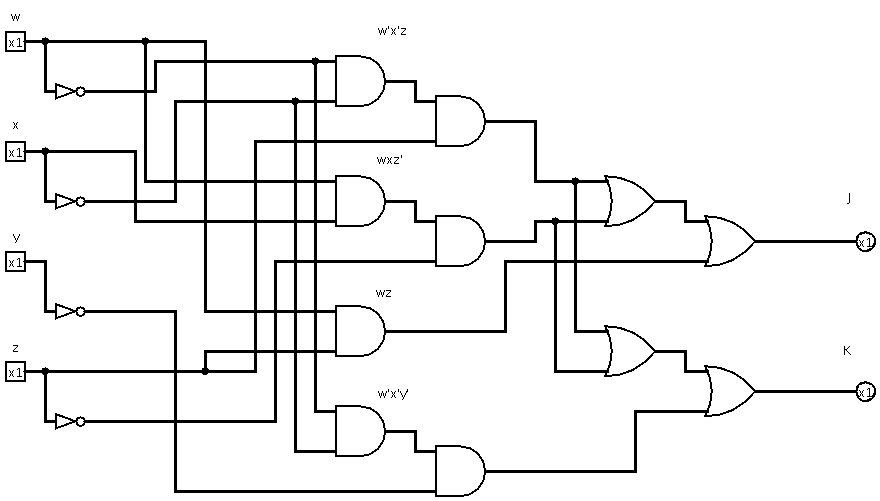
\includegraphics[scale=0.5]{JKjoint-01}
\caption{Circuit diagram of the jointly optimized solution of $J$ and $K$ when limited to two input gates.}
\label{fig:JKjointcircuit}
\end{figure}

Finally this jointly optimized solution (Figure \ref{fig:JKjointcircuit}
can be implemented in hardware using the 74HC04(NOT), 74HC08(AND),
and 74HC32(OR) gates.
Be sure to use pull down resistors (1k ohms works well) on the switch inputs
and to limit the current through the LED outputs with a 290 ohm resistor.
And if the LED outputs do not work try reversing their direction (remember
they behave like diodes).

\clearpage

\section{Observations}

The jointly optimized solution (Figure \ref{fig:JKjointcircuit}) of functions
$J$ and $K$ reproduced the expected truth table values (Table \ref{tbl:tt}).

The jointly optimized solution did reduce the number of gates
albeit slightly.
It can be seen from Table \ref{tbl:counts} that implementing
$J$ and $K$ independently resulted in 16 gates and 27 inputs.
Implementing these jointly resulted in 15 gates and 26 inputs,
a savings of 1 gate and 1 input.

\begin{table}[!htb]
\center
\begin{tabular}{cc}

\begin{tabular}{lll}
\multicolumn{3}{c}{\bf{$J$ by itself}} \\
gate type & \# gates & \# inputs\\
\hline
AND & 2 & 4\\
OR  & 1 & 2\\
NOT & 1 & 1 \\
\hline
\bf{TOTAL} & 4 & 7
\end{tabular}

&

\begin{tabular}{lll}
\multicolumn{3}{c}{\bf{$J$ and $K$ independently}} \\
gate type & \# gates & \# inputs\\
\hline
AND & 8 & 16 \\
OR  & 3 & 6  \\
NOT & 5 & 5  \\
\hline
\bf{TOTAL} & 16 & 27
\end{tabular}
\\
\\

\begin{tabular}{lll}
\multicolumn{3}{c}{\bf{$K$ by itself, 2 input gates}} \\
gate type & \# gates & \# inputs\\
\hline
AND & 6 & 12 \\
OR  & 2 & 4  \\
NOT & 4 & 4  \\
\hline
\bf{TOTAL} & 12 & 20
\end{tabular}

&

\begin{tabular}{lll}
\multicolumn{3}{c}{\bf{$J$ and $K$ jointly}} \\
gate type & \# gates & \# inputs\\
\hline
AND & 7 & 14 \\
OR  & 4 & 8  \\
NOT & 4 & 4  \\
\hline
\bf{TOTAL} & 15 & 26
\end{tabular}

\end{tabular} % outer formatting table

\caption{Metrics of gate and input counts for various configurations
of $J$ and $K$.}
\label{tbl:counts}
\end{table}


\section{Conclusion}

The lab was a success in developing a optimized hardware implementation
of two distinct logic functions.
The jointly optimized solution resulted in a slight, but still significant,
reduction in the number of gates and gate inputs.

% flush all the figures
%\clearpage

% Uncomment these if you have references,
%\pagebreak
%\renewcommand*{\refname}{\vspace{-8mm}}
%\section{References}
%%\bibliographystyle{plain}
%%\bibliographystyle{mslapa}
%\bibliographystyle{ieeetr}
%\bibliography{../references}

% Appendix (if needed)

\end{document}

% vim:foldmethod=marker
